\documentclass[12pt,a4paper]{ctexart}

\usepackage[a4paper,margin=2.4cm]{geometry}
\usepackage{amsmath,amssymb,bm}
\usepackage{booktabs}
\usepackage{enumitem}
\usepackage{graphicx}
\usepackage{tabularx}
\usepackage{hyperref}
\usepackage{physics}
\usepackage{setspace}
\usepackage{caption}
\usepackage{subcaption}
\usepackage{float}

\graphicspath{{figures/}}

\hypersetup{
	colorlinks=true,
	linkcolor=black,
	citecolor=blue,
	urlcolor=blue,
	pdftitle={无中微子双beta衰变课程论文},
	pdfauthor={原子核物理大作业}
}

\title{无中微子双\texorpdfstring{$\beta$}{beta}衰变}
\author{}
\date{\today}

\begin{document}

\maketitle

\begin{abstract}
无中微子双贝塔衰变（$0\nu\beta\beta$）是检验轻子数破坏和中微子 Majorana 性质的重要稀有核过程。双贝塔衰变的基本物理可从偶偶核质量关系和轻子数计数出发理解：$2\nu\beta\beta$ 是标准模型允许的轻子数守恒二阶弱过程，而 $0\nu\beta\beta$ 因末态缺少两个反中微子而具有 $\Delta L=2$。在实验上，前者对应电子总能量连续谱，后者对应 $Q_{\beta\beta}$ 附近的窄峰。若 $0\nu\beta\beta$ 由轻 Majorana 中微子交换主导，其衰变率与有效 Majorana 质量 $m_{\beta\beta}$ 有关，而 $m_{\beta\beta}$ 又依赖中微子质量排序和未知 Majorana 相位。进一步地，半衰期到粒子物理参数的解释需要核矩阵元作为关键输入。近期手征有效场论研究将 $0\nu\beta\beta$ 核矩阵元从 leading order 系统补全到 N$^2$LO，把长程项、短程接触项、超软中微子贡献和环图贡献统一纳入同一振幅，并显示 N$^2$LO 修正达到约 $5$--$15\%$，对未来半衰期解释不可忽略。
\end{abstract}

\noindent\textbf{关键词：}无中微子双贝塔衰变；轻子数破坏；Majorana 中微子；有效 Majorana 质量；手征有效场论；N$^2$LO

\tableofcontents

\newpage
\onehalfspacing

\section{引言}

\section{双贝塔衰变的基本物理}

\subsection{双贝塔衰变为什么会发生}

普通 $\beta^-$ 衰变可写为
\begin{equation}
	(A,Z)\rightarrow(A,Z+1)+e^-+\bar{\nu}_e .
\end{equation}
从核素图像看，它使质量数 $A$ 不变、电荷数 $Z$ 增加 1。若对某个固定 $A$ 的同量异位素链，母核 $(A,Z)$ 到中间奇奇核 $(A,Z+1)$ 的单贝塔衰变在能量上不允许，或由于角动量、宇称和核结构选择规则被强烈抑制，而母核到另一个偶偶核 $(A,Z+2)$ 的总质量差为正，则双贝塔衰变可以作为二阶弱过程发生：
\begin{equation}
	(A,Z)\rightarrow(A,Z+2)+2e^-+2\bar{\nu}_e .
	\label{eq:2nubb}
\end{equation}
这就是标准模型允许的双中微子双贝塔衰变（$2\nu\beta\beta$）。

这类过程常发生在偶偶核之间，原因是核配对效应会使偶偶核相对更稳定，而相邻奇奇核质量较高。以 $A=136$ 同量异位素链为例，$^{136}$Xe 到 $^{136}$Cs 的单贝塔路径不易发生，而到 $^{136}$Ba 的双贝塔路径可以能量允许。图 \ref{fig:a136} 中的质量关系直观展示了这一点。

\begin{figure}[htbp]
	\centering
	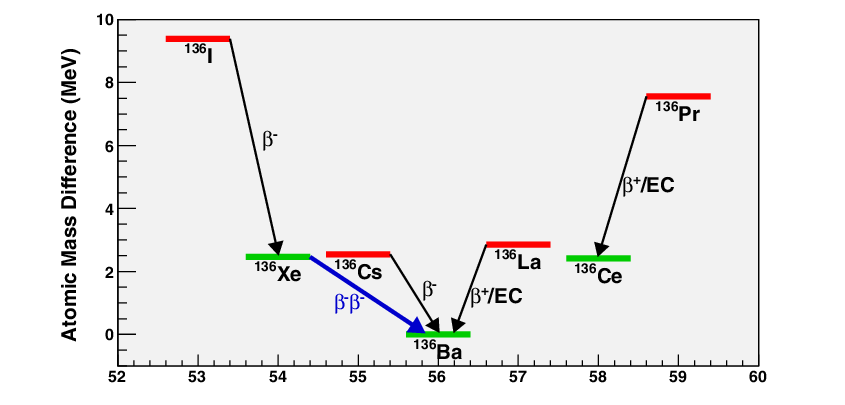
\includegraphics[width=0.72\textwidth]{fig6_A136_mass_crop.png}
	\caption{$A=136$ 同量异位素质量关系示意。偶偶核相对更稳定，中间奇奇核质量较高，使单贝塔路径受阻而双贝塔路径可发生（参考自文献\cite{GomezCadenas2023}）。}
	\label{fig:a136}
\end{figure}

从弱相互作用阶数看，$2\nu\beta\beta$ 可以理解为两个单贝塔顶点在同一原子核内同时发生。每个顶点满足标准模型带电流相互作用，整个过程保持总轻子数守恒。由于末态有两个电子和两个反中微子，四体相空间使该过程极其稀有，典型半衰期可达 $10^{18}$--$10^{21}$ 年量级，但它已经在多个核素中被观测到\cite{GomezCadenas2023}。因此，$2\nu\beta\beta$ 本身不是新物理信号，却为理解核波函数和检验双贝塔核模型提供了重要基准。

\subsection{\texorpdfstring{$2\nu\beta\beta$ 与 $0\nu\beta\beta$}{2nu beta beta 与 0nu beta beta} 的关键区别}

无中微子双贝塔衰变写作
\begin{equation}
	(A,Z)\rightarrow(A,Z+2)+2e^- .
	\label{eq:0nubb}
\end{equation}
它与式 \eqref{eq:2nubb} 的形式差别只是少了两个反中微子，但物理含义完全不同：$2\nu\beta\beta$ 是标准模型允许的轻子数守恒过程，而 $0\nu\beta\beta$ 是轻子数破坏过程。

取轻子数约定
\begin{equation}
	L(e^-)=+1,\qquad L(\nu_e)=+1,\qquad L(\bar{\nu}_e)=-1,
\end{equation}
原子核本身轻子数为零。于是对双中微子模式，
\begin{equation}
	L_f=2L(e^-)+2L(\bar{\nu}_e)=2-2=0=L_i,
\end{equation}
总轻子数守恒。对无中微子模式，
\begin{equation}
	L_f=2L(e^-)=2,\qquad L_i=0,
\end{equation}
所以
\begin{equation}
	\Delta L=L_f-L_i=+2 .
\end{equation}
文献中常写作 $|\Delta L|=2$，即轻子数破坏两个单位。这里的 ``2'' 来自末态有两个电子，每个电子都带 $+1$ 轻子数；在标准 $2\nu\beta\beta$ 中，两个反中微子的 $-2$ 正好抵消两个电子的 $+2$，而 $0\nu\beta\beta$ 没有这一抵消项。

因此，$0\nu\beta\beta$ 一旦被观测到，就不只是发现一种新的核衰变模式，而是直接说明自然界存在轻子数破坏过程。这一点是它在粒子物理和宇宙学中受到重视的根本原因：轻子数破坏与 Majorana 质量、跷跷板机制以及早期宇宙轻子生成机制都有潜在联系。

\subsection{实验信号：连续谱与单能峰}

实验不能直接 ``看见没有中微子''，真正测量的是两个电子的能量沉积。对 $2\nu\beta\beta$，两个反中微子会带走不可见能量，因此两个电子的总能量形成从 0 到 $Q_{\beta\beta}$ 的连续谱：
\begin{equation}
	0<E_{e1}+E_{e2}<Q_{\beta\beta}.
\end{equation}
对 $0\nu\beta\beta$，末态只有两个电子，理想情况下它们几乎带走全部衰变能：
\begin{equation}
	E_{e1}+E_{e2}\simeq Q_{\beta\beta}.
\end{equation}
因此，$0\nu\beta\beta$ 的实验信号是在 $Q_{\beta\beta}$ 附近的 ROI 中出现一个窄峰。探测器能量分辨率越好，该峰越窄，越容易和 $2\nu\beta\beta$ 谱尾以及环境本底区分。

\begin{figure}[htbp]
	\centering
	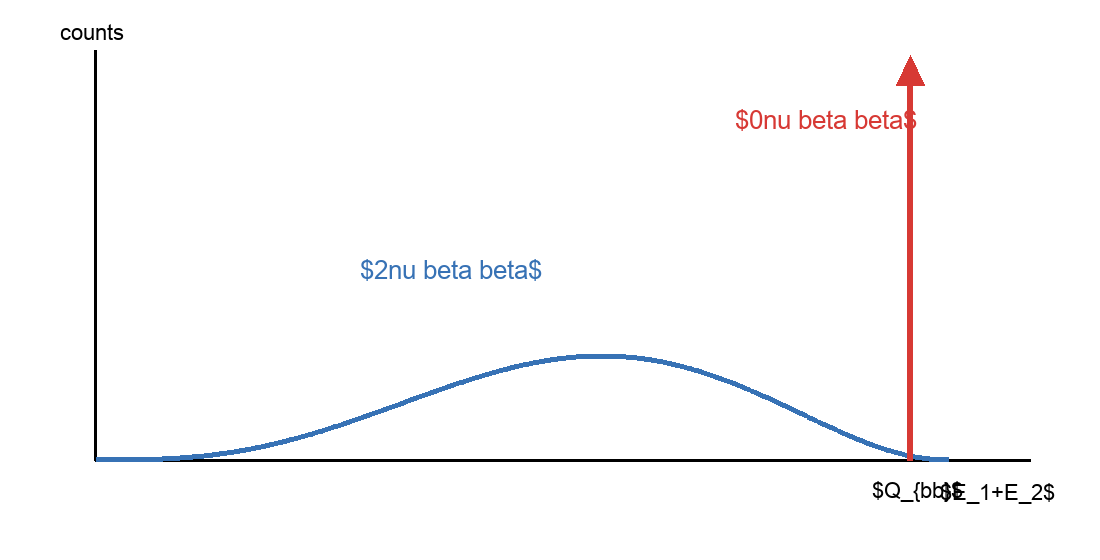
\includegraphics[width=0.72\textwidth]{spectrum.png}
	\caption{$2\nu\beta\beta$ 连续谱与 $0\nu\beta\beta$ 在 $Q_{\beta\beta}$ 处窄峰的示意图。}
	\label{fig:spectrum}
\end{figure}

实际实验中，峰会被能量分辨率展宽，本底来源包括天然放射性链中的 $\gamma$ 射线、表面 $\alpha$ 污染、宇宙线诱发事件、探测器材料放射性以及 $2\nu\beta\beta$ 连续谱尾部。高 $Q_{\beta\beta}$ 核素通常更有利，因为它们的相空间因子较大，且峰位可能避开部分天然 $\gamma$ 本底。候选核素还需要考虑天然丰度、同位素富集成本、探测器制备难度和 NME 理论可靠性。当前常见候选核素包括 $^{76}$Ge、$^{82}$Se、$^{100}$Mo、$^{130}$Te 和 $^{136}$Xe。

\subsection{本部分小结}

双贝塔衰变的基本物理可以概括为三点。第一，双贝塔衰变发生在某些单贝塔路径受阻而双贝塔路径能量允许的偶偶核中。第二，$2\nu\beta\beta$ 是标准模型允许的轻子数守恒过程，而 $0\nu\beta\beta$ 因末态没有两个反中微子而具有 $\Delta L=2$。第三，实验上 $2\nu\beta\beta$ 表现为电子总能量连续谱，$0\nu\beta\beta$ 表现为 $Q_{\beta\beta}$ 附近窄峰。上述内容为后续讨论 Majorana 中微子和有效质量提供了基础。

\section{Majorana 中微子与有效质量}

\subsection{Dirac 与 Majorana 问题}

中微子振荡实验已经证明至少两个中微子质量本征态具有非零质量，但振荡实验只能测量质量平方差和混合角，不能回答中微子是 Dirac 粒子还是 Majorana 粒子。对带电费米子来说，粒子和反粒子必然不同；但中微子不带电，因此原则上可以满足 Majorana 条件
\begin{equation}
	\nu=\nu^c,
\end{equation}
即中微子等同于自身的电荷共轭场。

Dirac 质量项需要同时存在左手和右手中微子场，并保持总轻子数守恒；Majorana 质量项则把中微子场与其电荷共轭场相连，会破坏轻子数两个单位。由于 $0\nu\beta\beta$ 正是 $\Delta L=2$ 过程，它天然与 Majorana 质量问题相联系。

在轻 Majorana 中微子交换机制中，两个弱顶点之间由虚中微子线连接。一个中子变成质子并放出电子和虚中微子；该虚中微子被另一个中子吸收，使其也变成质子并放出第二个电子。若中微子是 Majorana 粒子，产生的反中微子可以被视作中微子被另一个顶点吸收。由于标准弱相互作用只耦合左手中微子和右手反中微子，这条内部线需要手征翻转，而手征翻转由中微子质量提供。因此轻中微子交换振幅与中微子质量成正比。

\begin{figure}[htbp]
	\centering
	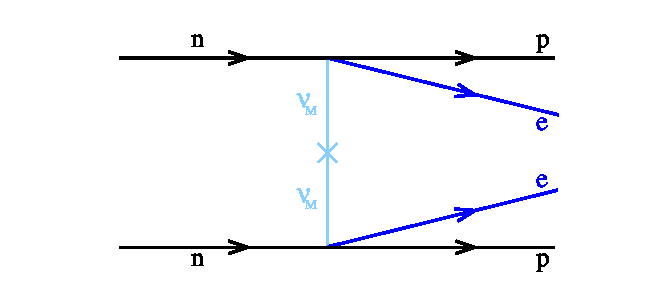
\includegraphics[width=0.62\textwidth]{fig2_light_nu_exchange_crop.png}
	\caption{轻 Majorana 中微子交换机制示意图。两个弱顶点由虚 Majorana 中微子传播子连接，手征翻转使振幅与中微子质量相关（参考自文献\cite{Engel2017}）。}
	\label{fig:lightnu}
\end{figure}

更一般地，在标准模型有效场论中，Majorana 质量可由五维 Weinberg 算符产生：
\begin{equation}
	\mathcal{L}_5=
	\frac{c_{\alpha\beta}}{\Lambda}
	\left(\overline{L_\alpha^c}\tilde{H}^{\ast}\right)
	\left(\tilde{H}^{\dagger}L_\beta\right)+{\rm h.c.},
\end{equation}
其中 $L_\alpha$ 是轻子双重态，$H$ 是 Higgs 双重态，$\Lambda$ 是新物理尺度。电弱对称性破缺后，
\begin{equation}
	(m_\nu)_{\alpha\beta}\sim \frac{c_{\alpha\beta}v^2}{\Lambda}.
\end{equation}
这说明即便新物理尺度远高于核物理能区，也可能通过低能轻子数破坏算符在 $0\nu\beta\beta$ 中留下可观测效应。

\subsection{有效 Majorana 质量的定义}

在标准轻中微子交换机制下，粒子物理部分通常由有效 Majorana 质量控制：
\begin{equation}
	m_{\beta\beta}
	=
	\left|\sum_{i=1}^{3}U_{ei}^{2}m_i\right|
	=
	|(m_\nu)_{ee}|.
	\label{eq:mbb}
\end{equation}
其中 $m_i$ 是三个中微子质量本征态的质量，$U_{ei}$ 是 PMNS 混合矩阵第一行元素，表示电子味中微子在第 $i$ 个质量本征态中的混合振幅。这个量等于中微子质量矩阵在电子味基下的 $(e,e)$ 元素的模。

需要注意，式 \eqref{eq:mbb} 中是 $U_{ei}^2$，不是 $|U_{ei}|^2$。因此不同质量本征态的贡献是相干叠加，复相位不能被消去。把 Majorana 相位显式写出，有
\begin{equation}
	m_{\beta\beta}
	=
	\left|
	m_1c_{12}^2c_{13}^2
	+m_2s_{12}^2c_{13}^2e^{i\alpha_{21}}
	+m_3s_{13}^2e^{i\alpha_{31}}
	\right|.
	\label{eq:mbb-expanded}
\end{equation}
这里 $s_{ij}=\sin\theta_{ij}$，$c_{ij}=\cos\theta_{ij}$，$\alpha_{21}$ 和 $\alpha_{31}$ 是 Majorana 相位。振荡实验可以测量混合角和质量平方差，但不能测量 Majorana 相位，也不能单独确定最轻中微子质量。因此 $m_{\beta\beta}$ 不是一个固定数值，而是一条随最轻质量和相位变化的允许带。

\subsection{质量排序与相位抵消}

有效质量的大小强烈依赖质量排序。正常排序（NO）满足
\begin{equation}
	m_1<m_2<m_3,
\end{equation}
其中 $m_1$ 最轻。此时三个质量本征态对 $m_{\beta\beta}$ 的贡献可能发生明显相消，尤其当 Majorana 相位取特定值时，$m_{\beta\beta}$ 可以很小，甚至在理论上接近零。倒置排序（IO）满足
\begin{equation}
	m_3<m_1<m_2,
\end{equation}
其中 $m_1$ 和 $m_2$ 较重且电子味成分较大，通常会给出十几 meV 量级的下界，不容易完全相消。

\begin{figure}[htbp]
	\centering
	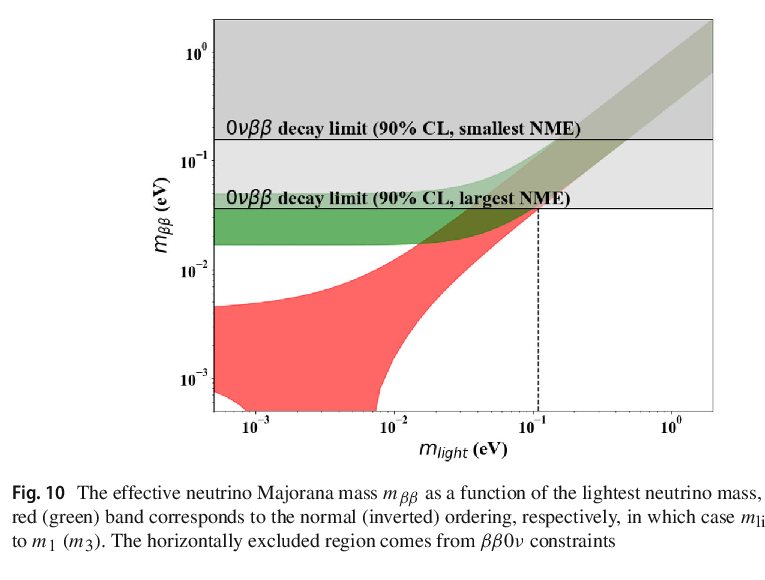
\includegraphics[width=0.74\textwidth]{fig_review_mbb_NO_IO.png}
	\caption{$m_{\beta\beta}$ 随最轻中微子质量变化的允许区域。红色和绿色带分别对应正常排序与倒置排序，灰色区域表示实验限制（数据取自文献\cite{GomezCadenas2023}）。}
	\label{fig:mbb}
\end{figure}

图 \ref{fig:mbb} 展示了 $m_{\beta\beta}$ 与最轻中微子质量的关系。横轴是最轻质量，纵轴是有效 Majorana 质量。带状区域的宽度来自未知 Majorana 相位和振荡参数误差。若未来实验灵敏度覆盖倒置排序区域而仍无信号，则可能意味着：中微子是 Dirac 粒子；或中微子是 Majorana 粒子但质量排序为正常且相位抵消强；或 $0\nu\beta\beta$ 的实际机制比单纯轻中微子交换更复杂。

\subsection{与其他质量观测量的关系}

$m_{\beta\beta}$ 不是唯一的中微子质量观测量。直接 $\beta$ 衰变实验（如 KATRIN）测量的是
\begin{equation}
	m_\beta=
	\left(\sum_i |U_{ei}|^2m_i^2\right)^{1/2}.
\end{equation}
宇宙学观测约束的是质量和
\begin{equation}
	\Sigma=m_1+m_2+m_3.
\end{equation}
这两个量都不依赖 Majorana 相位，也不直接检验轻子数破坏。相比之下，$m_{\beta\beta}$ 对 Majorana 相位敏感，并且只有在 $0\nu\beta\beta$ 这类 $\Delta L=2$ 过程中出现。因此，$0\nu\beta\beta$、直接质量测量、宇宙学约束和振荡实验是互补的。

\subsection{机制解释的谨慎性}

如果未来观测到 $0\nu\beta\beta$，它将强烈说明中微子具有 Majorana 性质。Schechter--Valle 黑箱定理表明，只要存在 $0\nu\beta\beta$，原则上就会诱导 Majorana 质量项\cite{SchechterValle1982}。但这并不意味着实际衰变率一定完全由轻中微子交换主导。右手流、重 Majorana 中微子、标量交换、超对称粒子或其他短程轻子数破坏机制也可能产生同样的两个电子末态。

因此，在轻中微子交换主导的假设下，半衰期可以转化为 $m_{\beta\beta}$；但若存在多个机制相干叠加，单个核素的半衰期不足以唯一确定粒子物理来源。未来若出现信号，还需要多核素测量、电子角关联、单电子能谱和多机制 NME 计算共同参与机制判别。

\section{半衰期公式与核矩阵元}

\subsection{标准半衰期公式与有效Majorana质量}

无中微子双贝塔衰变（$0\nu\beta\beta$）的半衰期是连接实验观测与粒子物理参数的核心纽带。在标准轻Majorana中微子交换机制主导的假设下，半衰期 $T_{1/2}^{0\nu}$ 的倒数可表示为几个因子的乘积~\cite{GomezCadenas2023,Engel2017}：
\begin{equation}
\left(T_{1/2}^{0\nu}\right)^{-1} = G^{0\nu}(Q,Z) \cdot g_A^4 \cdot \left| M^{0\nu} \right|^2 \cdot \left( \frac{m_{\beta\beta}}{m_e} \right)^2 \label{eq:halflife}
\end{equation}
该公式清晰地体现了问题的跨尺度性质。其中：
\begin{enumerate}
\item \textbf{相空间因子 $G^{0\nu}(Q,Z)$}：描述衰变释放的两个电子的相体积。它主要取决于衰变能 $Q_{\beta\beta}$ 和子核的原子序数 $Z$，可以通过量子电动力学(QCD)精确计算，不确定性很小~\cite{GomezCadenas2023}。
\item \textbf{轴矢耦合常数 $g_A$}：表征核子层次弱相互作用的强度。在自由核子中的值约为 $g_A \simeq 1.27$，但在核介质中会发生经验性的“淬灭”(quenching)修正，(通常降至约0.7-0.8 倍),以适应核模型对单 $\beta$和 $2\nu\beta\beta$衰变率的计算,因此其取值存在一定的不确定性。
\item \textbf{核矩阵元 $M^{0\nu}$}：描述衰变过程中初态 $(A,Z)$ 和末态 $(A,Z+2)$ 两个原子核波函数之间的跃迁振幅。它描述了强相互作用在核尺度上的复杂关联效应，不同核结构方法(如壳模型、QRPA、能量密度泛函等)给出的结果相差可达 2-3 倍,这也是从实验半衰期提取有效 Majorana 质量 $m_{\beta\beta}$的主要理论瓶颈。

\item \textbf{有效Majorana质量 $m_{\beta\beta}$}：这是粒子物理层面的目标参数。对于轻中微子交换机制，其定义为PMNS混合矩阵元和中微子质量本征值的组合：
\begin{equation}
m_{\beta\beta} = \left| \sum_{i=1}^{3} U_{ei}^2 m_i \right| \label{eq:meff}
\end{equation}
由于Majorana相位 $\alpha_i$ 的存在，$m_{\beta\beta}$ 可以是相长或相消干涉的结果，因此即使中微子是Majorana粒子，$m_{\beta\beta}$ 也可能非常小。
\end{enumerate}
从公式~\eqref{eq:halflife} 可知，一旦实验给出半衰期下限 $T_{1/2}^{0\nu} > T_{\mathrm{lim}}$，即可反推出 $m_{\beta\beta}$ 的上限：
\begin{equation}
m_{\beta\beta} < \frac{m_e}{g_A^2 |M^{0\nu}|} \sqrt{\frac{1}{G^{0\nu} T_{\mathrm{lim}}}} \label{eq:mlimit}
\end{equation}
这表明，核矩阵元 $M^{0\nu}$ 的计算精度直接决定了从实验极限提取 $m_{\beta\beta}$ 上限的可靠性，或未来发现信号时确定中微子质量尺度的准确性。

\subsection{核矩阵元的复杂结构}

$0\nu\beta\beta$ 的核矩阵元远比单 $\beta$ 衰变复杂，因为它涉及两个核子同时发生弱相互作用，并通过交换一个虚中微子耦合。从微观有效理论出发，核矩阵元可分解为费米（Fermi, F）、伽莫夫-泰勒（Gamow-Teller, GT）和张量（Tensor, T）三项的贡献~\cite{Engel2017,GomezCadenas2023}：
\begin{equation}
M^{0\nu} = M_{GT}^{0\nu} - \left(\frac{g_V}{g_A}\right)^2 M_{F}^{0\nu} + M_T^{0\nu} \label{eq:Mdecomp}
\end{equation}
在长程轻中微子交换机制下，这些分量的具体形式可写为两体算符在初、末态核波函数之间的期望值：
\begin{equation}
M_{K}^{0\nu} = \frac{2R}{\pi} \langle \Psi_f | \sum_{m<n} \tau_m^+ \tau_n^+ \int_0^\infty j_\lambda(q r_{mn}) \frac{h_K(q^2)}{q + \bar{E} - (E_i+E_f)/2} \mathcal{O}_K(m,n) \, dq \, | \Psi_i \rangle \label{eq:Mlong}
\end{equation}
其中 $R$ 是核半径，$\tau^+$ 是同位旋升算符，$j_\lambda(q r)$ 是球贝塞尔函数（$\lambda=0$ 对应 $F$ 和 $GT$ 项，$\lambda=2$ 对应 $T$ 项），$r_{mn}$ 是两核子间的距离，$\bar{E}$ 是闭合近似下的平均激发能。算符 $\mathcal{O}_K$ 对 $F$ 项为单位算符 $\mathbb{I}$，对 $GT$ 项为 $\sigma_m\cdot\sigma_n$，对 $T$ 项为张量算符 $S_{mn}=3(\hat{r}\cdot\sigma_m)(\hat{r}\cdot\sigma_n)-\sigma_m\cdot\sigma_n$。中微子势 $h_K(q^2)$ 包含了矢量、轴矢、弱磁和赝标量形状因子，体现了弱流在核子层次的复杂结构。

\subsection{核矩阵元：从基本输入到主要瓶颈}

$0\nu\beta\beta$ 衰变的特殊之处在于，其虚中微子传递的典型动量 $q\sim 100-200\ \mathrm{MeV}$，远大于核低能激发能，却与核子内部的费米动量尺度相当。因此，NME 的计算对核波函数的细节极为敏感，尤其是短程核关联、形变、对关联以及同位旋混合等效应。

对 $^{76}\mathrm{Ge}$、$^{136}\mathrm{Xe}$ 等中重核，完整求解核多体问题在计算上极具挑战。当前主要采用包括核壳模型（SM）、准粒子无规相位近似（QRPA）、能量密度泛函理论结合生成坐标法（EDF-GCM）以及相互作用玻色子模型（IBM）等不同方法~\cite{Engel2017}。这些方法在模型空间、有效相互作用和处理集体关联的方式上各有取舍，导致对同一核素的 $M^{0\nu}$ 预测值存在约2–3倍的差异~\cite{GomezCadenas2023}。这种巨大的理论不确定性，直接转化为从半衰期反推 $m_{\beta\beta}$ 时近一个数量级的不确定性，已成为当前制约 $0\nu\beta\beta$ 物理潜力的最主要理论瓶颈。如下图所示为使用不同方法计算同一核素的核矩阵元时出现的不同数值。
\begin{figure}[htbp]
	\centering
	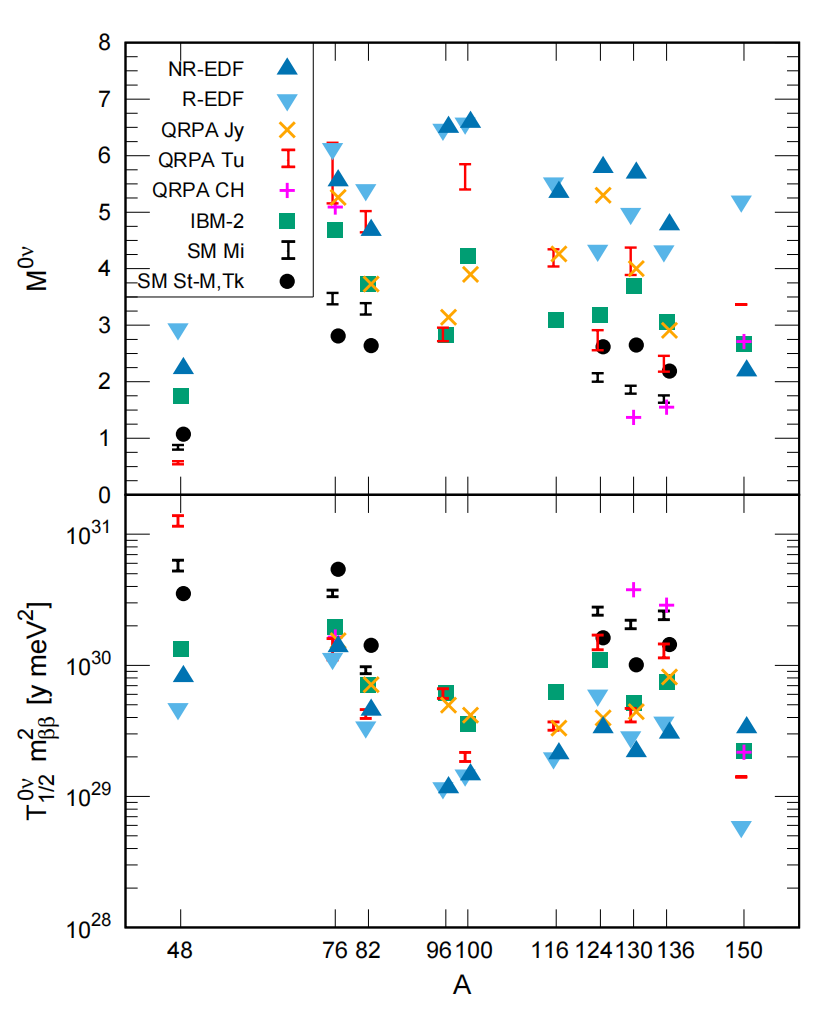
\includegraphics[width=0.72\textwidth]{the_limit_of_NME_section4.png}
	\caption{不同核结构方法计算的 $0\nu\beta\beta$ 核矩阵元 $M^{0\nu}$ 的比较。不同方法在同一核素上给出相差约 2-3 倍的结果，反映了理论不确定性的严重程度（数据取自文献\cite{GomezCadenas2023}）。}
	\label{fig:NME}
\end{figure}

此外，普遍存在于核模型中的 $g_A$ 淬灭问题（即计算出的单 $\beta$ 和 $2\nu\beta\beta$ 跃迁强度普遍大于实验值）也为 $0\nu\beta\beta$ 的预测蒙上阴影。淬灭的根源可能来自模型空间截断导致的多体关联缺失，也可能来自 $\Delta$ 共振态等非核子自由度的贡献~\cite{Engel2017}。理解其物理本质并统一处理其在 $0\nu\beta\beta$ 中的影响，是当前核理论研究的核心课题之一。

\section{实验研究现状}

从实验角度看，$0\nu\beta\beta$ 的核心目标是在极低本底条件下寻找 $Q_{\beta\beta}$ 附近的单能峰。若实验未观测到显著峰形超额，则给出半衰期下限；若未来观测到信号，则需要进一步结合能谱、事件拓扑和多核素结果排除未知本底。由式 \eqref{eq:halflife} 可知，实验可直接约束的是 $T_{1/2}^{0\nu}$，而其对 $m_{\beta\beta}$ 的解释还依赖相空间因子、$g_A$ 以及核矩阵元 $M^{0\nu}$。因此，实验研究现状不能只看探测器灵敏度，也必须联系理论矩阵元的不确定性。

\subsection{实验信号与灵敏度指标}

对 $2\nu\beta\beta$，两个反中微子会带走一部分不可见能量，因此两个电子总能量形成连续谱；对 $0\nu\beta\beta$，末态只有两个电子，理想情况下两电子总能量集中在 $Q_{\beta\beta}$ 附近。实验上的感兴趣区间（region of interest, ROI）通常围绕 $Q_{\beta\beta}$ 选取，其宽度由探测器能量分辨率决定。能量分辨率越好，ROI 越窄，连续谱尾部和环境 $\gamma$ 本底越容易被压低。

实验灵敏度主要由候选核素数目、测量时间、探测效率、能量分辨率和本底指数共同决定。粗略地说，候选核质量越大、运行时间越长，潜在信号事件数越多；而本底越低、能量分辨率越高，对同一半衰期的排除能力越强。实际实验中还必须同时控制天然放射性链中的 $\gamma$ 射线、表面 $\alpha$ 污染、宇宙线诱发事件、材料内禀放射性以及 $2\nu\beta\beta$ 谱尾等背景。正因为 $0\nu\beta\beta$ 半衰期可能达到 $10^{26}$ 年以上，现代实验通常需要在深地下环境中长期运行，并对探测器材料进行严格筛选。

更定量地说，若候选同位素质量为 $M_{\rm iso}$，摩尔质量为 $W$，同位素丰度或富集度为 $a$，探测效率为 $\varepsilon$，测量时间为 $t$，则给定半衰期下的期望信号数可写为
\begin{equation}
	N_{0\nu}
	=
	\ln 2\,
	\frac{N_A}{W}\,
	aM_{\rm iso}\,
	\varepsilon t\,
	\frac{1}{T_{1/2}^{0\nu}} ,
	\label{eq:expected-events}
\end{equation}
其中 $N_A$ 为阿伏伽德罗常数。若 ROI 中的本底期望数为
\begin{equation}
	B=b\,\Delta E\,M_{\rm iso}t ,
	\label{eq:background-index}
\end{equation}
这里 $b$ 是本底指数，$\Delta E$ 是能量窗口宽度，则在有本底情形下半衰期灵敏度近似随曝光量和本底按
\begin{equation}
	T_{1/2}^{0\nu}
	\propto
	\frac{a\varepsilon}{W}
	\sqrt{\frac{M_{\rm iso}t}{b\Delta E}}
	\label{eq:background-limited-sensitivity}
\end{equation}
增长；在近零本底极限下则近似正比于总曝光量 $M_{\rm iso}t$。这解释了为什么下一代实验同时追求吨级同位素、窄 ROI 和近零本底。

\subsection{国际主要技术路线}

目前国际上尚无被普遍确认的 $0\nu\beta\beta$ 信号，但多个实验已经把典型候选核素的半衰期下限推进到 $10^{25}$--$10^{26}$ 年量级，下一代实验则以 $10^{27}$--$10^{28}$ 年量级为目标~\cite{Dolinski2019,Agostini2023,GomezCadenas2023}。由于大质量、低本底、高能量分辨率和事件拓扑重建难以由单一技术同时达到，国际上形成了多路线并行发展的格局。

\begin{table}[htbp]
	\centering
	\caption{无中微子双贝塔衰变主要实验路线概览}
	\label{tab:experiment-routes}
	\begin{tabularx}{\textwidth}{p{2.8cm}p{2.6cm}p{2.4cm}X}
		\toprule
		技术路线 & 代表实验 & 候选核素 & 主要特点 \\
		\midrule
		高纯锗探测器 & GERDA、MAJORANA、LEGEND & $^{76}$Ge & 能量分辨率极好，本底水平低；向吨级扩展时同位素富集和探测器规模是关键挑战。\\
		液体闪烁体 & KamLAND-Zen、SNO+ & $^{136}$Xe、$^{130}$Te & 可装载大质量同位素，曝光量优势明显；能量分辨率相对较弱，需要依赖低本底和统计量。\\
		氙时间投影室 & EXO、nEXO、NEXT & $^{136}$Xe & 可同时获得能量和位置信息，气体 TPC 还可利用双电子拓扑鉴别本底；系统工程复杂。\\
		低温量热器 & CUORE、CUPID & $^{130}$Te、$^{100}$Mo & 能量分辨率较好，可通过热光双读出进行粒子鉴别；低温大阵列运行要求高。\\
		\bottomrule
	\end{tabularx}
\end{table}

高纯锗路线以 $^{76}$Ge 作为源和探测器本身，优势是出色的能量分辨率和成熟的低本底技术。液体闪烁体路线能够溶入或装载大量候选核素，KamLAND-Zen 对 $^{136}$Xe 的搜索给出了非常强的半衰期限制，是当前最具代表性的结果之一~\cite{GomezCadenas2023}。氙 TPC 路线同样以 $^{136}$Xe 为重要候选核，液氙方案强调大质量和三维定位，气氙方案则更重视电子径迹拓扑信息。低温量热器路线将候选核素嵌入晶体中，通过低温下的热信号测量沉积能量，CUORE 和 CUPID 分别代表了该路线的当前与未来发展方向。

这些路线的互补性非常重要。若未来某一核素或某一技术首先观测到峰形超额，仍需要其他核素和其他探测技术进行交叉验证；若多个核素给出相互一致的半衰期关系，则不仅能增强发现可信度，也有助于区分轻中微子交换、右手流或短程轻子数破坏算符等不同机制。

\subsection{国内相关平台与发展方向}

国内在 $0\nu\beta\beta$ 方向的布局主要依托深地下低本底环境、大型氙探测技术和大型液体闪烁体平台~\cite{Wang2024}。中国锦屏地下实验室（CJPL）具有极深岩石覆盖和极低宇宙线通量，是开展稀有事例搜索的重要基础设施。对 $0\nu\beta\beta$ 而言，深地下环境可以显著降低宇宙线诱发本底，为 CDEX、PandaX 以及未来可能的低本底双贝塔衰变实验提供平台条件。

PandaX 系列实验以大型氙时间投影室为核心技术，最初主要面向暗物质直接探测，但氙 TPC 技术与 $^{136}$Xe 的 $0\nu\beta\beta$ 搜索天然相关。若未来发展到更大质量、更低本底并充分利用事件位置与拓扑信息，氙 TPC 路线有望在国内 $0\nu\beta\beta$ 搜索中发挥重要作用。江门中微子实验 JUNO 则是大型液体闪烁体平台，主要物理目标是确定中微子质量顺序和精确测量振荡参数；从技术储备看，大质量液闪探测器也为未来装载双贝塔候选核素提供了可能性。

总体来看，国内实验优势并不局限于某一个装置，而体现在低本底环境、探测器工程和中微子物理平台的组合。未来若能与核矩阵元理论、同位素富集和材料纯化技术协同推进，将有机会在下一代 $0\nu\beta\beta$ 搜索中形成有竞争力的实验布局。

\section{研究进展一：格点 QCD}

核矩阵元的不确定性是解释 $0\nu\beta\beta$ 半衰期的主要理论瓶颈。传统核多体方法从核子自由度出发，需要有效相互作用、弱流算符和有限模型空间近似；而这些输入最终都来源于低能强相互作用。格点 QCD（lattice QCD, LQCD）的意义在于，它从夸克和胶子自由度出发，在离散欧氏时空中非微扰地计算 QCD 路径积分，为少体弱过程和核有效场论低能常数提供第一性原理输入。

\subsection{格点 QCD 在 \texorpdfstring{$0\nu\beta\beta$}{0nu beta beta} 中的角色}

真实实验候选核如 $^{76}$Ge、$^{130}$Te 和 $^{136}$Xe 都是中重核，当前还无法直接从夸克胶子层面计算其完整 $0\nu\beta\beta$ 核矩阵元。格点 QCD 更现实的作用，是先计算可控的少强子或少核子过程，例如 $\pi^-\to\pi^+ee$、$\Sigma^-\to\Sigma^+ee$ 和 $nn\to pp\,ee$，再通过核有效场论把这些少体结果匹配成低能常数，最终输入到核多体计算中。

Davoudi 等人的工作首次在多核子体系中计算与长程轻 Majorana 中微子交换相关的 $0\nu\beta\beta$ 振幅~\cite{Davoudi2024}。该工作关注的核心过程是
\begin{equation}
	nn\rightarrow pp\,ee,
\end{equation}
并同时计算统计性质更好的
\begin{equation}
	\Sigma^-\rightarrow \Sigma^+ee
\end{equation}
作为方法检验。需要强调的是，这些过程并不是直接对应某个实际中重核的完整衰变，而是用于隔离少体强子动力学和提取 EFT 输入的理论计算对象。

\subsection{从弱哈密顿量到强子振幅}

在远低于电弱尺度的能区，单次 $d\to u$ 弱跃迁可由四费米弱哈密顿量描述：
\begin{equation}
	H_W
	=2\sqrt{2}G_FV_{ud}
	(\bar u_L\gamma^\mu d_L)
	(\bar e_L\gamma_\mu\nu_{eL})
	+\mathrm{h.c.}.
	\label{eq:lqcd-hw}
\end{equation}
这里 $G_F$ 是费米常数，$V_{ud}$ 是 CKM 矩阵元，$J_\mu=\bar u_L\gamma_\mu d_L$ 是夸克层面的左手弱流。$0\nu\beta\beta$ 需要两个中子变成两个质子，因此振幅来自两次 $H_W$ 插入。若由轻 Majorana 中微子交换主导，中微子传播子中手征翻转带来有效 Majorana 质量 $m_{\beta\beta}$，而其余复杂性集中在两个弱流之间的强子矩阵元中。

\begin{figure}[htbp]
	\centering
	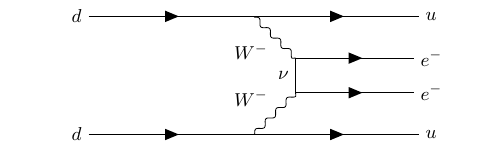
\includegraphics[width=0.56\textwidth]{lqcd_long_distance_diagram.png}
	\caption{长程轻 Majorana 中微子交换机制的夸克层面示意图。两个 $d$ 夸克分别经弱流转化为 $u$ 夸克，中间由轻 Majorana 中微子传播子连接（裁取自文献\cite{Davoudi2024}）。}
	\label{fig:lqcd-long-distance-diagram}
\end{figure}

将已知的弱相互作用常数、电子态归一化和 $m_{\beta\beta}$ 因子剥离后，可定义目标强子振幅
\begin{equation}
	A_{i\to f}
	\equiv
	\frac{M_{i\to f}}
	{4G_F^2V_{ud}^2m_{\beta\beta}N_{e1}N_{e2}} .
	\label{eq:lqcd-amp-def}
\end{equation}
插入完整中间强子态后，该振幅可写成
\begin{equation}
	A_{i\to f}
	=
	\sum_n
	\frac{
	\langle N_f|J_\mu(0)|n\rangle
	\langle n|J^\mu(0)|N_i\rangle
	}{
	2\tilde E_n|\mathbf q|
	\left(|\mathbf q|+\tilde E_n-E_i+m_e\right)
	}.
	\label{eq:lqcd-amp-sum}
\end{equation}
式中 $N_i$ 和 $N_f$ 分别表示初态和末态强子系统，在核心通道中对应 $nn$ 和 $pp$；$|n\rangle$ 是所有可能的中间强子态；$\mathbf q$ 是虚中微子三动量。这个表达式清楚地显示，LQCD 要解决的不是 $G_F$ 或 $m_{\beta\beta}$ 的问题，而是强相互作用体系对两个弱流插入的响应。

\subsection{由欧氏关联函数提取矩阵元}

格点 QCD 的实际计算对象是欧氏关联函数。二点函数
\begin{equation}
	C_2(t')
	=
	\int d^3x_f\,
	\langle 0|
	O_i(\mathbf x_f,t_f)
	O_i^\dagger(0,t_i)
	|0\rangle
	\label{eq:lqcd-c2}
\end{equation}
用于提取初态或末态强子系统的基态能量和插值算符重叠因子。含有 $0\nu\beta\beta$ 信息的是四点函数
\begin{equation}
	C_4^{i\to f}
	(t_{\rm snk},t,t_{\rm src})
	=
	\int d^3x_f\,d^3x\,d^3y\,
	D(x-y)
	\langle 0|
	O_f(x_f)
	J_\mu(x)J^\mu(y)
	O_i^\dagger(0)
	|0\rangle ,
	\label{eq:lqcd-c4}
\end{equation}
其中 $D(x-y)$ 是轻中微子传播子，$O_i^\dagger$ 和 $O_f$ 分别在源端和汇端产生、投影强子外态。为了约去普通传播因子和重叠因子，文献\cite{Davoudi2024}构造比值
\begin{equation}
	R_{i\to f}
	=
	\frac{
	C_4^{i\to f}
	(t_{\rm snk},t,t_{\rm src})
	}{
	C_2(t_{\rm snk}+|t|+t_{\rm src})
	}.
	\label{eq:lqcd-ratio}
\end{equation}
在源端和汇端时间距离足够大时，激发态污染被指数压低；再对两个弱流之间的时间间隔积分，即可得到
\begin{equation}
	A_{i\to f}
	=
	2E_0
	\int_{-\infty}^{\infty}dt\,
	\lim_{t_{\rm src},t_{\rm snk}\to\infty}
	R_{i\to f}(t_{\rm snk},t,t_{\rm src}) .
	\label{eq:lqcd-integral}
\end{equation}
这条关系把谱分解中的中间态求和转化为可数值计算的欧氏四点函数，是 LQCD 计算长程 $0\nu\beta\beta$ 强子振幅的关键。

在实际拟合中，去除外态激发态后得到的 $R_{i\to f}(t)$ 可在当前统计精度下近似写成单指数形式
\begin{equation}
	R_{i\to f}(t)\simeq A^{(R)}e^{-E^{(R)}|t|},
	\label{eq:lqcd-single-exp}
\end{equation}
于是式 \eqref{eq:lqcd-integral} 化为
\begin{equation}
	A_{i\to f}
	\simeq
	4E_0\,\frac{A^{(R)}}{E^{(R)}} .
	\label{eq:lqcd-single-exp-integral}
\end{equation}
这里 $A^{(R)}$ 和 $E^{(R)}$ 分别是比值函数的有效振幅和有效能隙。该近似对应于用主导中间态指数衰减描述两个弱流之间的欧氏时间依赖。

\subsection{数值结果、限制与物理意义}

文献\cite{Davoudi2024}的计算使用单一格点间距和单一体积，并在非物理夸克质量下进行，对应 $m_\pi=806~\mathrm{MeV}$。作者在有限体积中去除了中微子空间零模，以避免中间态能量导致的欧氏时间指数增长问题。通过二点函数提取 $\Sigma$ 和双中子能量，再由四点函数比值拟合并积分，得到重整化后的核心结果
\begin{align}
	a^2A_{\Sigma^-\to\Sigma^+} &= 0.00595(58),\\
	a^2A_{nn\to pp} &= 0.078(16).
\end{align}
其中 $a$ 是格点间距。$\Sigma$ 通道统计误差较小，$nn\to pp$ 通道噪声更大，但仍给出了多核子体系中长程 $0\nu\beta\beta$ 振幅的首个直接 LQCD 数值结果。

\begin{figure}[htbp]
	\centering
	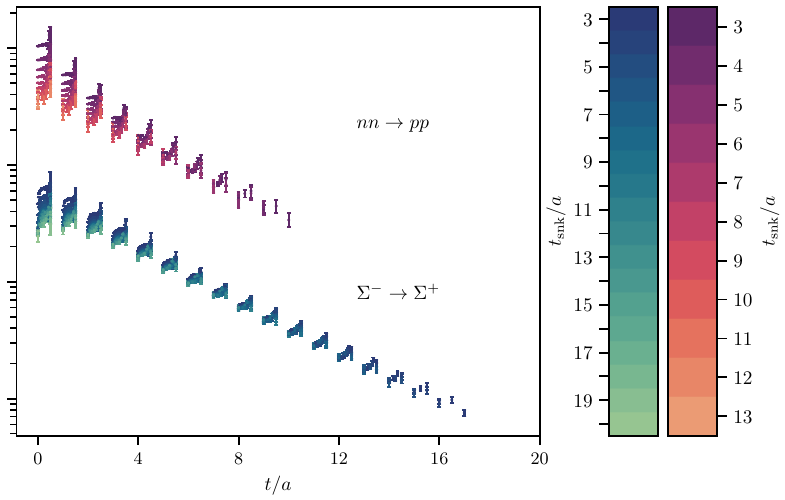
\includegraphics[width=0.72\textwidth]{lqcd_ratio_results.png}
	\caption{四点函数与二点函数比值 $R_{i\to f}$ 随两个弱流时间间隔 $t/a$ 的变化。上方数据对应 $nn\to pp$，下方数据对应 $\Sigma^-\to\Sigma^+$；指数衰减行为用于提取式 \eqref{eq:lqcd-single-exp-integral} 中的强子振幅（裁取自文献\cite{Davoudi2024}）。}
	\label{fig:lqcd-ratio-results}
\end{figure}

该结果目前不能直接用于真实实验核素的半衰期解释。主要限制包括：夸克质量远重于物理值，只有一个格点间距和体积，有限体积两核子谱以及到物理点的外推仍需进一步控制。然而它的重要性在于证明了多核子 $0\nu\beta\beta$ 相关矩阵元可以从 QCD 第一性原理出发计算。未来若能在接近物理夸克质量下同时计算 $nn\to pp$ 振幅和两核子散射参数，就有望匹配出 pionless EFT 或手征 EFT 中的短程低能常数，如 $g_\nu^{NN}$，从而降低重核 NME 计算中的模型依赖。

因此，格点 QCD 在整个 $0\nu\beta\beta$ 研究链条中的位置可以概括为
\begin{equation}
	\mathrm{QCD}
	\rightarrow
	\mathrm{few\mbox{-}body\ amplitudes}
	\rightarrow
	\mathrm{EFT\ low\mbox{-}energy\ constants}
	\rightarrow
	M^{0\nu}
	\rightarrow
	T_{1/2}^{0\nu}.
\end{equation}
它不是替代所有核多体方法，而是为核多体方法提供更可靠的底层输入。

\section{研究进展二：手征 EFT 到 N\texorpdfstring{$^2$}{2}LO}

\subsection{为什么需要手征 EFT}

实验测量或限制的是 $0\nu\beta\beta$ 半衰期，而半衰期与中微子质量参数之间需要核矩阵元连接。在轻 Majorana 中微子交换主导的标准情形中，通常有
\begin{equation}
	\left(T_{1/2}^{0\nu}\right)^{-1}
	=
	G^{0\nu}g_A^4|M^{0\nu}|^2
	\left|\frac{m_{\beta\beta}}{m_e}\right|^2 .
	\label{eq:half-life}
\end{equation}
这里 $G^{0\nu}$ 是相空间因子，$g_A$ 是轴矢耦合常数，$M^{0\nu}$ 是核矩阵元。相空间因子相对可控，而 $M^{0\nu}$ 依赖复杂核多体波函数和弱流算符，是把半衰期解释为 $m_{\beta\beta}$ 的主要理论瓶颈。

传统 NME 计算主要关注轻中微子交换导致的长程 neutrino potential。对这一部分，常写成
\begin{equation}
	M^{0\nu}
	=
	M_{GT}^{0\nu}
	-
	\left(\frac{g_V}{g_A}\right)^2M_F^{0\nu}
	+M_T^{0\nu},
\end{equation}
其中 $M_{GT}$、$M_F$ 和 $M_T$ 分别是 Gamow--Teller、Fermi 和 tensor 分量。这种分解说明 NME 不是单一常数，而包含自旋、同位旋、张量结构和核内动量传递。

手征有效场论（chiral effective field theory, $\chi$EFT）的作用，是把低能强相互作用、弱流和轻子数破坏算符放在同一个系统展开中。核内 $0\nu\beta\beta$ 的典型动量传递约为
\begin{equation}
	q\sim100~{\rm MeV},
\end{equation}
低于手征破缺尺度
\begin{equation}
	\Lambda_\chi\sim1~{\rm GeV}.
\end{equation}
因此可以按小参数 $q/\Lambda_\chi$ 组织算符。EFT 的价值不是简单给一个新数值，而是回答：哪些项应该在同一精度下一起保留，哪些过去被忽略的项应视为同阶修正，并评估遗漏项的不确定度。

\subsection{N\texorpdfstring{$^2$}{2}LO 工作的目标与对象}

文献\cite{Castillo2025}系统计算了重核中 $0\nu\beta\beta$ NME 完整到 next-to-next-to-leading order（N$^2$LO）的贡献。文献\cite{Castillo2025}考虑的核素包括
\begin{equation}
	^{76}{\rm Ge},\quad ^{82}{\rm Se},\quad ^{100}{\rm Mo},\quad
	^{130}{\rm Te},\quad ^{136}{\rm Xe},
\end{equation}
这些都是当前或下一代实验关注的主要候选核。

文献同时使用两类典型核多体方法：
\begin{itemize}[leftmargin=2em]
	\item pnQRPA，即 proton--neutron quasiparticle random phase approximation，适合描述电荷交换中间态，模型空间较大，但对粒子--粒子相互作用参数等较敏感；
	\item NSM，即 nuclear shell model，在有限价空间中能够较充分处理核子关联，但模型空间较小，高能轨道可能缺失。
\end{itemize}
两种方法并用的意义在于：如果某个 EFT 修正在两种核结构截断下表现一致，则其结果更稳健；如果符号或大小显著不同，则说明该修正对中间态结构或模型空间处理敏感。

\subsection{N\texorpdfstring{$^2$}{2}LO 半衰期公式}

文献\cite{Castillo2025}采用的核心公式为
\begin{equation}
	\left(t_{1/2}^{0\nu}\right)^{-1}
	=
	G^{0\nu}g_A^4
	\frac{m_{\beta\beta}^2}{m_e^2}
	\left|
	M_L^{0\nu}
	+M_S^{0\nu}
	+M_{\rm usoft}^{0\nu}
	+M_{\rm loop}^{0\nu}
	\right|^2 .
	\label{eq:n2lo-half-life}
\end{equation}
其中各项含义如下：
\begin{itemize}[leftmargin=2em]
	\item $M_L^{0\nu}$：LO 长程轻中微子交换项，是传统 NME 的主体；
	\item $M_S^{0\nu}$：LO 短程接触项，描述两个弱顶点在短距离上发生时的贡献；
	\item $M_{\rm usoft}^{0\nu}$：N$^2$LO 超软中微子贡献，对中间核态能量显式敏感；
	\item $M_{\rm loop}^{0\nu}$：N$^2$LO 环图贡献，包括不能吸收到核子形式因子中的部分。
\end{itemize}

这条公式有两个要点。第一，四类 NME 是在振幅中相干相加，而不是把 LO 结果乘以一个经验修正因子，所以不同项之间可能相长或相消。第二，在文献\cite{Castillo2025}采用的 $\chi$EFT power counting 中，LO 之后下一批新的独立 $0\nu\beta\beta$ NME 贡献出现在 N$^2$LO，因此公式中没有单独的 NLO NME 项。这不是说所有 EFT 问题都没有 NLO，而是轻中微子交换机制在这一计数下如此。

\subsection{LO 长程项与 LO 短程项}

LO 长程项对应通常的 light-neutrino exchange neutrino potential，可写为
\begin{equation}
	M_L^{0\nu}
	=
	M_{GT}^{0\nu}
	-
	\left(\frac{g_V}{g_A}\right)^2M_F^{0\nu}
	+M_T^{0\nu}.
\end{equation}
其中 Gamow--Teller 项通常最重要，Fermi 项由同位旋结构决定，tensor 项一般较小但不能先验忽略。传统 NME 计算的核心通常就是这个长程项及其相关的核模型处理。

短程项 $M_S^{0\nu}$ 则来自两个弱顶点距离很近时的接触贡献。早期 power counting 中，短程项曾被视为较高阶修正；但重整化一致性表明，为使理论可重整化，相关短程 NME 需要提升到 LO。它的强度由低能常数如 $g_{NN\nu}$ 控制，而这些常数不能直接从普通单贝塔衰变数据中确定，需要格点 QCD、轻核从头算或 EFT 匹配提供约束。

这说明 ``短程'' 并不等于 ``数值上很小''。在文献\cite{Castillo2025}的结果中，$M_S^{0\nu}$ 在若干核素中达到 $M_L^{0\nu}$ 的相当比例，特别是在 pnQRPA 中更明显。因此，只保留传统长程项会低估理论结构的复杂性。

\subsection{N\texorpdfstring{$^2$}{2}LO ultrasoft 项}

N$^2$LO 的第一类新增贡献来自 ultrasoft neutrinos。这里的 ``ultrasoft'' 指虚中微子动量远低于核 Fermi 动量。与 LO 长程项常用闭合近似不同，ultrasoft 项显式依赖中间核的 $1^+$ 态能量。它的结构使得中间态谱和 Gamow--Teller 强度分布直接影响 NME。

这点非常重要，因为它解释了为什么 pnQRPA 和 NSM 对 ultrasoft 项给出不同符号。NSM 在有限价空间中处理关联较充分，但可能缺少部分高能轨道；pnQRPA 模型空间较大，适合电荷交换中间态，但对参数和高能贡献较敏感。ultrasoft 项正好放大了这种中间态处理差异。

文献\cite{Castillo2025}中的 running sum 图（图 \ref{fig:running}）显示，$^{76}$Ge 的 ultrasoft NME 在较低中间态激发能区域，两种方法趋势较接近；但在约 $8$--$13$ MeV 区间，pnQRPA 出现显著抵消和符号变化，而 NSM 没有相同行为。这说明 N$^2$LO 差异不是简单的整体归一化差异，而来自中间态累积方式。

\begin{figure}[htbp]
	\centering
	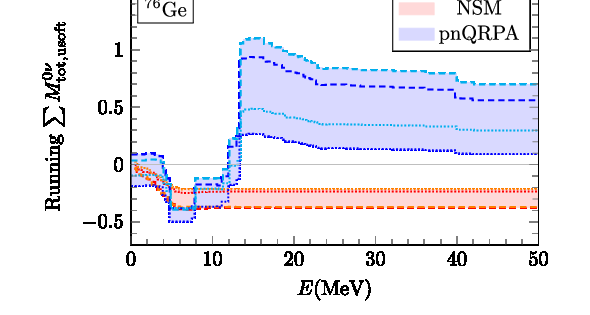
\includegraphics[width=0.82\textwidth]{eft_fig1_running_crop.png}
	\caption{$^{76}$Ge 的 total ultrasoft NME 随中间 $1^+$ 态激发能的 running sum（数据取自文献\cite{Castillo2025}）。pnQRPA 与 NSM 在 $8$--$13$ MeV 区间出现明显不同。}
	\label{fig:running}
\end{figure}

\subsection{N\texorpdfstring{$^2$}{2}LO loop 项}

N$^2$LO 的另一类贡献来自 loop diagrams。它们可分解为矢量--矢量（VV）、轴矢--轴矢（AA）和接触项（CT）等部分。不同 loop 分量之间可以相互抵消，例如某些核素中 VV 项与 AA、CT 项符号相反。由于 loop 项具有较强短程性质，它对 regulator、短程关联和重整化尺度较敏感。

这类贡献通常小于 LO 长程项，但仍可达到几个百分点到十几个百分点。更重要的是，它揭示了传统 ``核子形式因子修正'' 不能吸收全部 N$^2$LO 信息，部分环图必须作为独立 NME 计算。对未来高精度解释而言，loop 项的不确定性需要与短程低能常数、短程关联处理和多体模型误差一起估计。

\subsection{Table 1 的数值结果}

文献\cite{Castillo2025}的 Table 1 给出各核素在 pnQRPA 和 NSM 中的 LO 长程、LO 短程、N$^2$LO ultrasoft 和 N$^2$LO loop-soft 中心值及范围。图 \ref{fig:eft-table} 展示了该表的主要结果。

\begin{figure}[htbp]
	\centering
	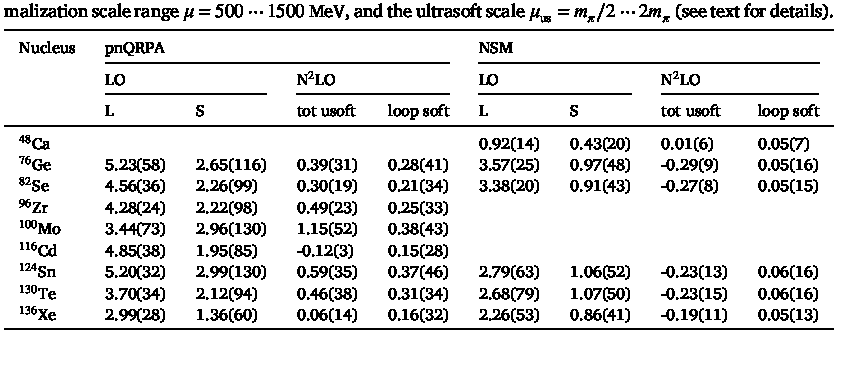
\includegraphics[width=0.9\textwidth]{eft_table1_crop.png}
	\caption{文献\cite{Castillo2025} Table 1 中的 NME 结果。表中列出 LO 长程项、LO 短程项、N$^2$LO total ultrasoft 和 N$^2$LO loop-soft。}
	\label{fig:eft-table}
\end{figure}

为了便于讨论，选取 $^{76}$Ge 和 $^{136}$Xe 的中心值列于表 \ref{tab:n2lo-examples}。
\begin{table}[htbp]
	\centering
	\caption{部分核素中 LO 与 N$^2$LO NME 中心值示例\cite{Castillo2025}}
	\label{tab:n2lo-examples}
	\begin{tabular}{lcccc}
		\toprule
		核素与方法 & $M_L$ & $M_S$ & $M_{\rm usoft}$ & $M_{\rm loop}^{\rm soft}$ \\
		\midrule
		$^{76}$Ge, pnQRPA & 5.23 & 2.65 & 0.39 & 0.28 \\
		$^{76}$Ge, NSM & 3.57 & 0.97 & $-0.29$ & 0.05 \\
		$^{136}$Xe, pnQRPA & 2.99 & 1.36 & 0.06 & 0.16 \\
		$^{136}$Xe, NSM & 2.26 & 0.86 & $-0.19$ & 0.05 \\
		\bottomrule
	\end{tabular}
\end{table}

从表中可读出三点。第一，$M_L$ 仍然是主导贡献，但 $M_S$ 并不小，尤其在 pnQRPA 中可达到长程项的相当比例。第二，N$^2$LO 项通常小于 LO，但已达到几个百分点到十几个百分点，不适合简单忽略。第三，$M_{\rm usoft}$ 在 pnQRPA 和 NSM 中常出现相反符号，这是文献\cite{Castillo2025}的重要发现之一。表中的 $M_{\rm loop}^{\rm soft}$ 是总环图贡献 $M_{\rm loop}^{0\nu}$ 中 soft-loop 部分的汇总，用于和 total ultrasoft 项分开比较。

以 $^{76}$Ge 为例，若粗略用表中中心值估算 N$^2$LO 相对 LO 的大小，
\begin{align}
	{\rm pnQRPA:}\quad
	\frac{M_{\rm usoft}+M_{\rm loop}^{\rm soft}}{M_L+M_S}
	&\simeq
	\frac{0.39+0.28}{5.23+2.65}
	\simeq 8.5\%,\\
	{\rm NSM:}\quad
	\frac{M_{\rm usoft}+M_{\rm loop}^{\rm soft}}{M_L+M_S}
	&\simeq
	\frac{-0.29+0.05}{3.57+0.97}
	\simeq -5.3\%.
\end{align}
这与文献摘要中的总体结论一致：NSM 中 N$^2$LO 修正中心值约为 $-(5\text{--}10)\%$，pnQRPA 中约为 $+(10\text{--}15)\%$。

\subsection{Ultrasoft 与 non-closure correction}

传统 $0\nu\beta\beta$ NME 计算常用闭合近似，即把中间态能量替换为平均闭合能量。闭合近似之外的修正通常称为 non-closure correction。文献\cite{Castillo2025}比较了 total ultrasoft NME 与 non-closure correction，发现两者量级相近，如图 \ref{fig:nonclosure} 所示。

\begin{figure}[htbp]
	\centering
	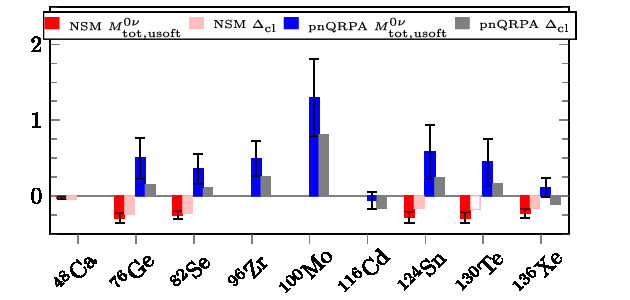
\includegraphics[width=0.82\textwidth]{eft_fig2_nonclosure_crop.png}
	\caption{Total ultrasoft NME 与 non-closure correction 的比较（参考自文献\cite{Castillo2025}）。二者量级相近，说明 N$^2$LO ultrasoft 项不是形式上的小修正。}
	\label{fig:nonclosure}
\end{figure}

这一结果的意义在于，它把传统核结构语言和 EFT 语言连接起来。过去 non-closure correction 常被视为核模型技术修正；在 $\chi$EFT 中，ultrasoft neutrino contribution 是按阶数出现的 N$^2$LO 项。二者同量级说明，若未来要实现高精度 NME 计算，不能只停留在闭合近似的 LO neutrino potential，而需要系统纳入 ultrasoft 项。

\subsection{物理意义与总结}

手征 EFT 到 N$^2$LO 的工作表明，现代 $0\nu\beta\beta$ NME 研究正在从 ``模型给一个数'' 转向 ``按 EFT 阶数系统补全算符和误差''。文献\cite{Castillo2025}的主要结论可概括为：
\begin{align}
	{\rm NSM:}\quad &\Delta_{\rm N^2LO}\sim -(5\text{--}10)\%,\\
	{\rm pnQRPA:}\quad &\Delta_{\rm N^2LO}\sim +(10\text{--}15)\%.
\end{align}
N$^2$LO 修正虽非主导项，但已经达到下一代实验解释不能随意忽略的量级。

更重要的是，pnQRPA 与 NSM 的符号差异说明，不同多体方法之间的差异不只体现在总 NME 大小上，也体现在中间态 running sum 和高阶修正的符号上。未来若要降低理论误差，需要进一步理解中间态谱、短程低能常数、regulator 依赖和两体弱流的影响。对于从实验半衰期提取 $m_{\beta\beta}$ 而言，N$^2$LO 的 $5$--$15\%$ NME 修正会转化为有效质量约束中的系统误差，因此必须纳入严肃的理论误差预算。

\section{研究进展三：MR-CDFT 多机制 NME}

\subsection{研究目标与动机}

当下一代实验将灵敏度推进至 $10^{27-28}$ 年量级时，一旦发现信号，首要问题便是：是什么机制驱动了 $0\nu\beta\beta$ 衰变？仅知道半衰期不足以判断背后的物理机制。标准的光Majorana中微子交换，和非标准机制(如右手流，重中微子等)都可能导致相同的两个电子末态。由 Ding、Li 和 Yao 于 2024 年发表的论文《Nuclear matrix elements of neutrinoless double-beta decay in covariant density functional theory with different mechanisms》~\cite{Ding2024} 正是为回答这一问题而开展的系统性理论研究。

该工作的核心目标是：在手征有效场论的框架下，采用统一的多参考协变密度泛函理论（MR-CDFT）波函数，系统地计算五个重要候选核素（$^{76}\mathrm{Ge}$、$^{82}\mathrm{Se}$、$^{100}\mathrm{Mo}$、$^{130}\mathrm{Te}$、$^{136}\mathrm{Xe}$）在标准以及多种非标准机制下的组合核矩阵元，并探讨不同核模型不确定性对新物理参数约束的影响。

\subsection{理论框架：三种机制与组合NME}

该研究在手征EFT的指导下，将 Leading-order 的轻子数破坏跃迁势分为三类~\cite{Ding2024}：
\begin{itemize}
\item \textbf{Type-I（标准机制）}：由轻Majorana中微子交换主导，其强度由有效质量 $m_{\beta\beta}$ 控制。
\item \textbf{Type-II（长程非标准机制）}：来源于动量依赖的长程 LNV 相互作用，对应不同的洛伦兹结构。
\item \textbf{Type-III（短程机制）}：由高能新物理（如重中微子交换）在低能标下产生的接触相互作用主导。
\end{itemize}
\begin{figure}[htbp]
	\centering
	\subcaptionbox{Type-I：标准轻Majorana中微子交换机制\cite{Ding2024}}{
		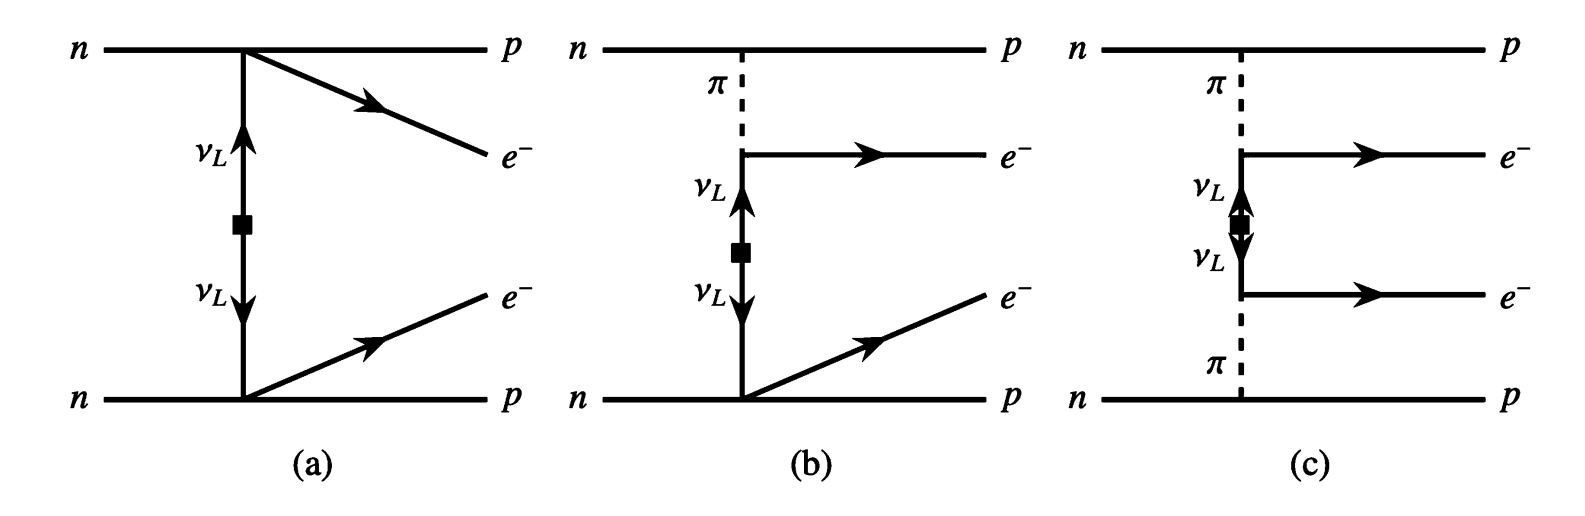
\includegraphics[width=0.8\textwidth]{type1.png}
	}
	
	\subcaptionbox{Type-II：长程非标准机制\cite{Ding2024}}{
		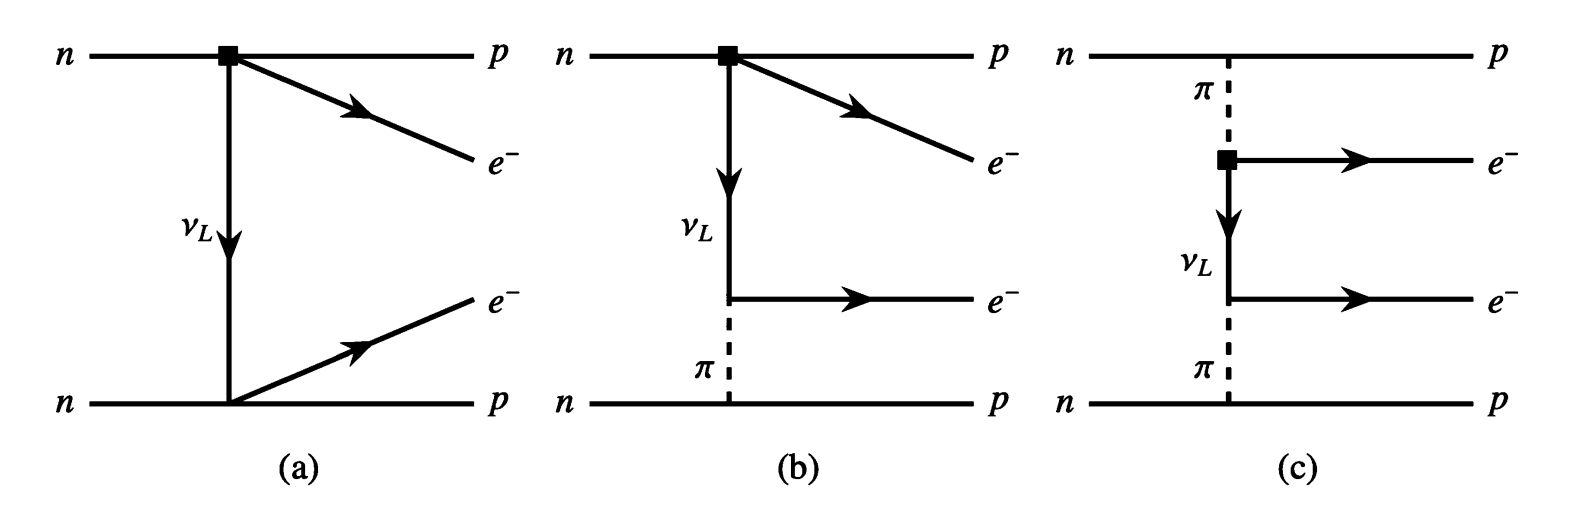
\includegraphics[width=0.8\textwidth]{type2.png}
	}
	
	\subcaptionbox{Type-III：短程机制\cite{Ding2024}}{
		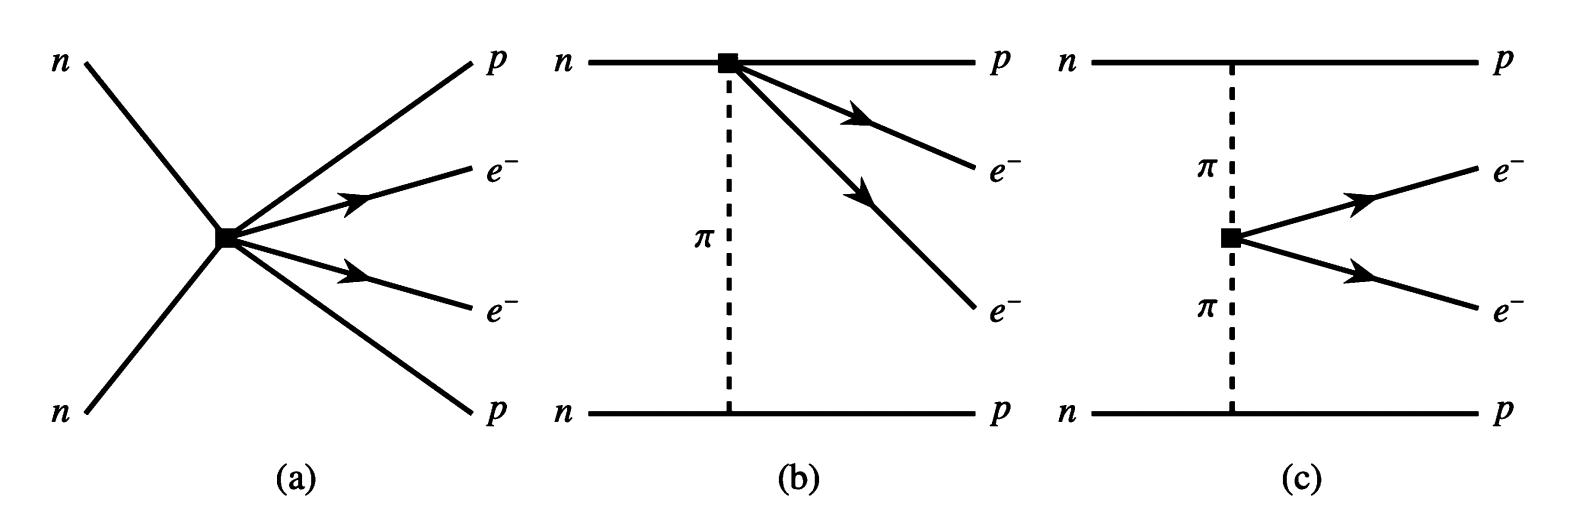
\includegraphics[width=0.8\textwidth]{type3.png}
	}
	\caption{Ding et al.~\cite{Ding2024}中考虑的三类 $0\nu\beta\beta$ 机制示意图。Type-I 是标准的轻Majorana中微子交换；Type-II 是长程非标准机制；Type-III 是短程机制。每类机制对应不同的费曼图结构和核矩阵元组合。}
	\label{fig:mechanisms}
\end{figure}
NME 不是单一数值，而是需要根据具体机制和轻子结构（$L,R,m_e,E,M$）进行组合。例如，标准机制的振幅 $\mathcal{A}_L$ 被表示为：
\begin{equation}
\begin{aligned}
\mathcal{A}_L = \frac{m_{\beta\beta}}{m_e}&\left(M_L^{\mathrm{I,NN}} + M_L^{\mathrm{I},\pi N} + M_L^{\mathrm{I},\pi\pi}\right) \\
&+ \sum_i C_i^{\mathrm{II,III}} M_i^{\mathrm{II,III}}
\end{aligned}
\label{eq:Alarge}
\end{equation}
其中 $M_i^{a}$ 是基础 Fermi、GT 和 Tensor NME 的特定线性组合，而 $C_i$ 是待定的无量纲 LNV 系数。因此，计算的关键在于首先获得基础 NME 分量，再按机制需求进行组合。

\subsection{MR-CDFT 方法及其优势}

MR-CDFT 是一种处理中重核集体关联的强大工具。它从相对论点耦合密度泛函 PC-PK1 出发，通过以下几个步骤构建初、末态 $0^+$ 波函数~\cite{Ding2024}：
\begin{enumerate}
\item \textbf{约束平均场计算}：生成一系列具有不同形变（四极、八极等）的参考态。
\item \textbf{对称性恢复}：对每个参考态进行角动量和粒子数投影，得到具有确定好量子数的态。
\item \textbf{生成坐标混合}：将投影后的态作为基矢，通过求解 Hill-Wheeler 方程进行组态混合，从而描述集体关联和形状共存。
\end{enumerate}
相较于传统的壳模型或 QRPA，MR-CDFT 能够更自然地处理中重核中普遍存在的形变效应，并在统一的框架下自洽地描述母核与子核，这使其成为计算多核素、多机制 NME 的理想平台。

\subsection{主要结论与意义}

该研究的主要发现和贡献可以概括为以下几点。

\textbf{组合NME的模型依赖性。}虽然单个NME分量在不同模型中差异巨大，但按特定费曼图组合后的 NME 在一定程度上缩小了分歧。然而，对于 $^{136}\mathrm{Xe}$，不同模型（MR-CDFT, SM, sQRPA, IBM2）给出的组合NME仍存在约2–4倍的差异（见文献~\cite{Ding2024} 图4），表明非标准机制的核不确定性丝毫不亚于标准机制。

\begin{figure}[htbp]
	\centering
	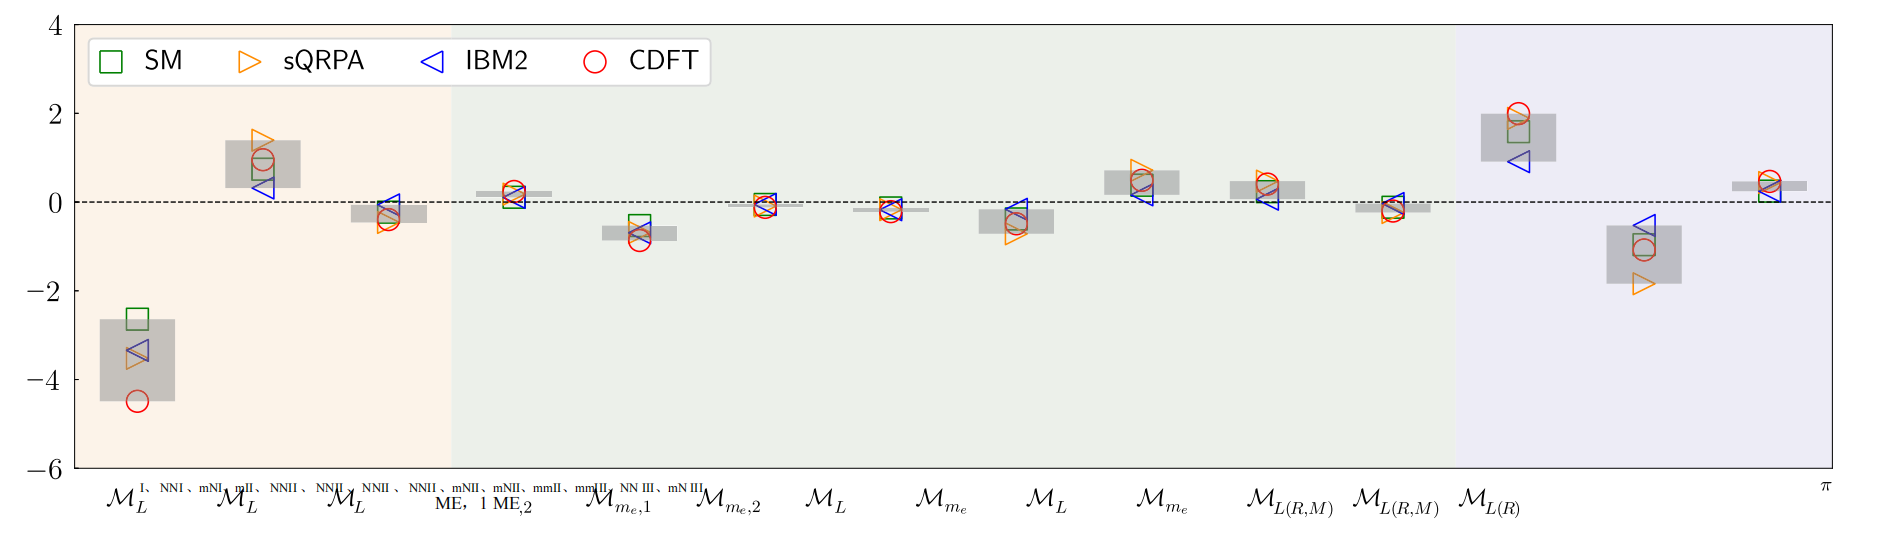
\includegraphics[width=0.85\textwidth]{Ding-fig4.png}
	\caption{文献\cite{Ding2024}不同核模型对 $^{136}\mathrm{Xe}$ 的组合NME比较。}
	\label{fig:ding-comparison}
\end{figure}

\textbf{对新物理参数的约束。}利用 KamLAND-Zen 实验对 $^{136}\mathrm{Xe}$ 的最新半衰期下限，该工作推导了 $m_{\beta\beta}/m_e$ 及各 LNV 系数 $C_i$ 的上限。结果显示，MR-CDFT 由于其预测的 NME 值通常较大，因而给出了最为严格的参数空间限制（见文献~\cite{Ding2024} 图5）。

\begin{figure}[htbp]
	\centering
	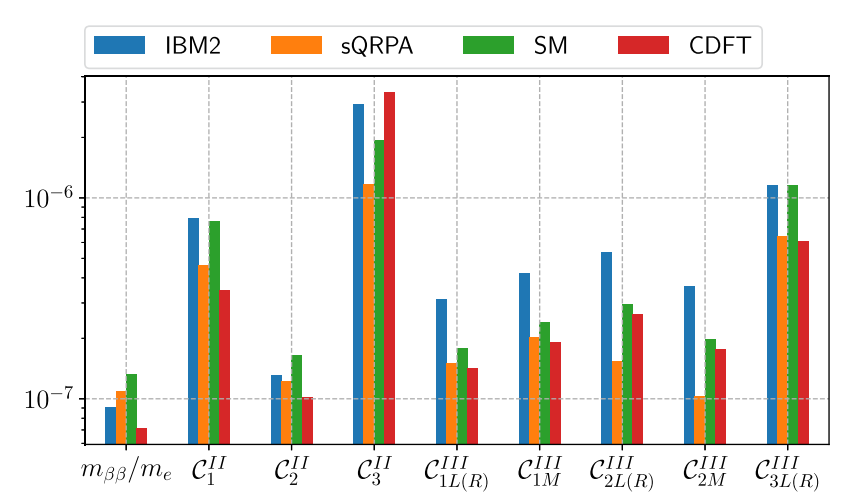
\includegraphics[width=0.85\textwidth]{Ding-fig5.png}
	\caption{文献\cite{Ding2024}不同核模型对 LNV 系数的约束比较。}
	\label{fig:ding-constraints}
\end{figure}

\textbf{机制间的相干效应。}研究系统分析了标准机制与非标准机制之间的干涉图样。例如，与振幅 $\mathcal{A}_L$ 贡献相关的系数（如 $C_{3L}^{\mathrm{II}}$）与 $m_{\beta\beta}$ 呈现出线性相关，而与 $\mathcal{A}_{m_e}$ 等贡献相关的系数则呈现出椭圆状的相关区域（见文献~\cite{Ding2024} 图6）。这种相关性分析为未来通过多观测量联合分析来甄别新物理机制提供了理论依据。

\begin{figure}[H]
	\centering
	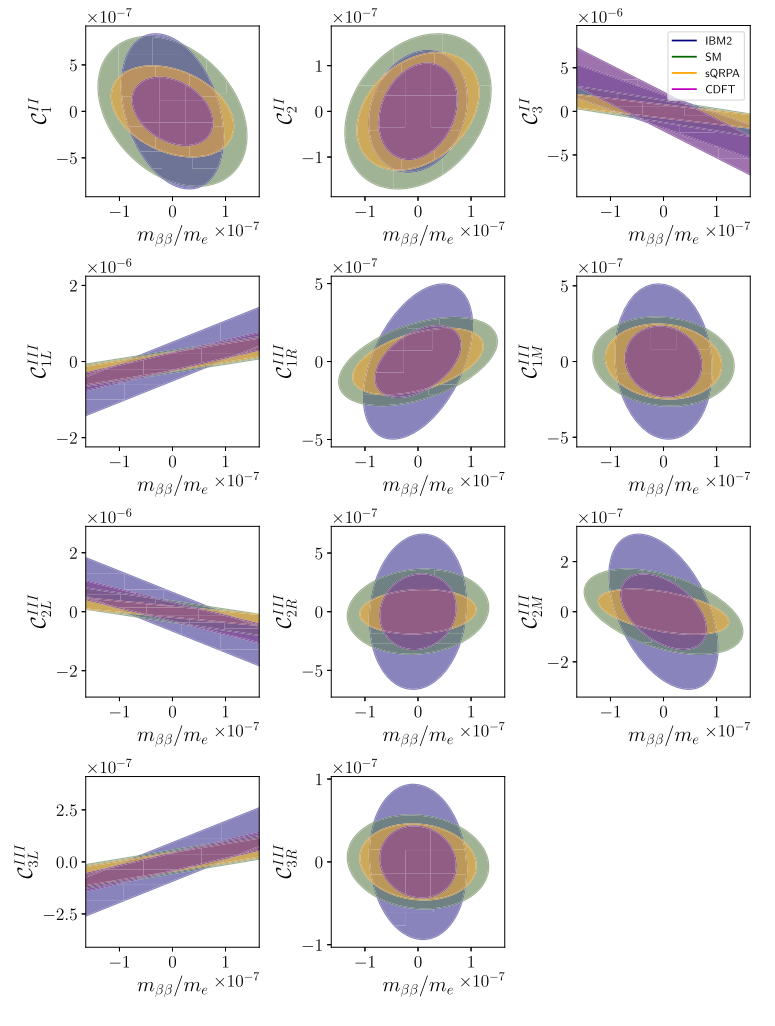
\includegraphics[width=0.85\textwidth]{Ding-fig6.png}
	\caption{文献\cite{Ding2024}LNV 系数之间的相关性分析。}
	\label{fig:ding-correlation}
\end{figure}

\textbf{连接理论与实验。}该工作不仅计算了 NME，还将低能 LNV 系数与 SMEFT 的 Wilson 系数联系起来，从而建立了从核实验半衰期到高能新物理尺度 $\Lambda$ 的映射。

\textbf{小结：}Ding 等人的工作代表了当前 $0\nu\beta\beta$ 理论研究的先进水平。它不仅是单纯的计算 NME，而是构建了一个连接“特定新物理模型 – 手征EFT算符 – 核多体波函数 – 实验观测量”的完整链条。该研究的核心信息是：未来一旦发现信号，仅凭一个核素的半衰期无法区分机制，必须依赖多核素测量、对干涉项的分析以及多个核模型的交叉验证，而 MR-CDFT 为此提供了重要的理论工具。
\section{当前关键问题与展望}

\subsection{实验侧：从排除极限走向发现灵敏度}

当前 $0\nu\beta\beta$ 实验的首要挑战仍然是极端稀有性。若半衰期处于 $10^{27}$--$10^{28}$ 年量级，即使吨级同位素也只能期待非常少的信号事件。因此，未来实验必须同时推进四个方向：更大的候选核质量、更长的稳定运行时间、更低的本底水平以及更好的能量分辨率。任何一个因素不足，都会限制对倒置质量排序区域或更低 $m_{\beta\beta}$ 区域的覆盖。

另一个关键问题是信号确认。$Q_{\beta\beta}$ 附近的峰形超额可能来自真正的 $0\nu\beta\beta$，也可能来自未识别的放射性本底、表面污染或探测器响应效应。因此，未来的发现需要多层次验证：同一实验内部要依靠空间分布、事件拓扑和时间稳定性检验；不同实验之间要依靠多核素、多技术路线的交叉确认。只有当不同候选核素给出与核矩阵元预期相容的结果时，才能把峰形信号可靠解释为轻子数破坏过程。

\begin{figure}[htbp]
	\centering
	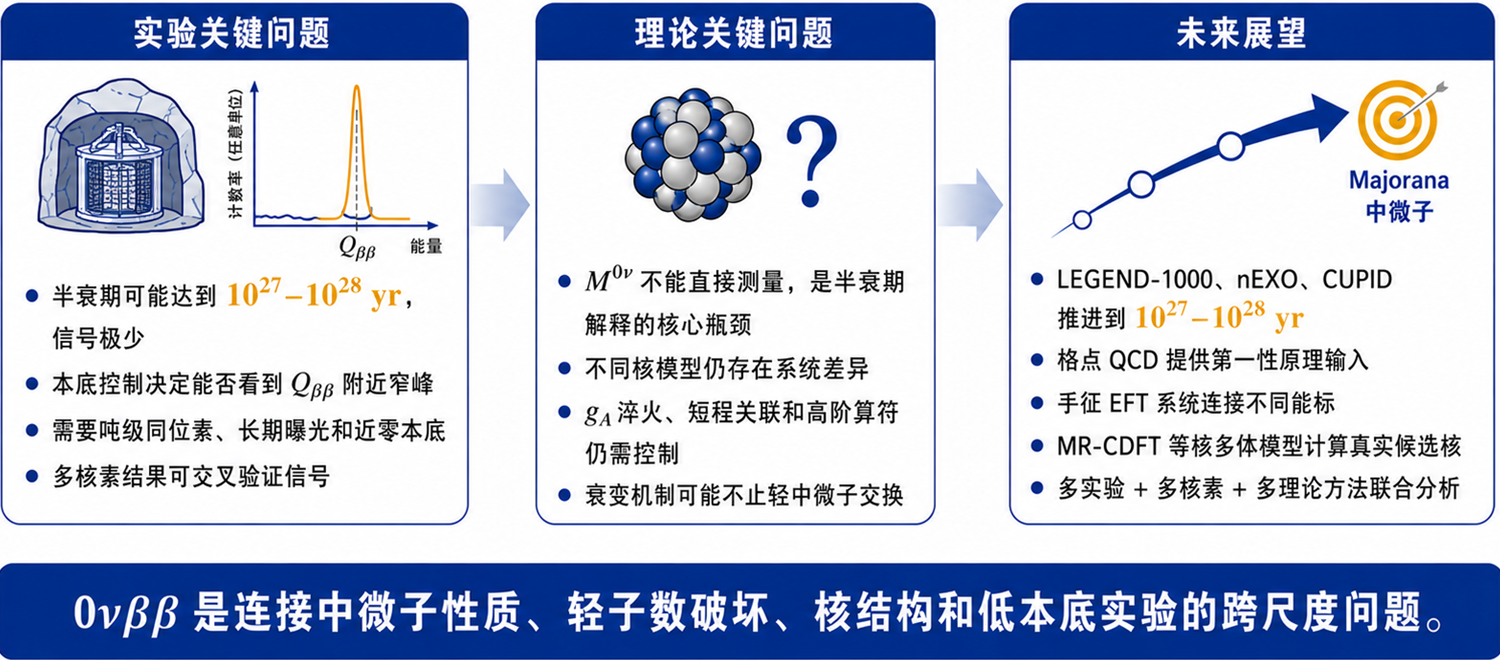
\includegraphics[width=0.92\textwidth]{outlook_key_issues.png}
	\caption{$0\nu\beta\beta$ 研究中的实验问题、理论问题与未来路线。实验侧关注能否在极低本底中发现 $Q_{\beta\beta}$ 附近窄峰，理论侧关注如何用可靠 NME 解释半衰期，未来则需要多实验、多核素和多理论方法联合推进（根据课程展示材料整理）。}
	\label{fig:outlook-key-issues}
\end{figure}

\subsection{理论侧：核矩阵元与低能常数}

理论方面，最大的瓶颈仍是核矩阵元 $M^{0\nu}$ 的不确定性。不同核结构方法对同一核素的预测可相差约 $2$--$3$ 倍，这会直接影响从半衰期到 $m_{\beta\beta}$ 或其他新物理耦合的反推。$g_A$ 淬灭、短程关联、核形变、模型空间截断、同位旋恢复以及两体弱流等问题，都可能改变 NME 的大小和误差预算。

未来降低理论不确定性的方向不是单纯选择某一个模型，而是建立跨尺度的统一框架。格点 QCD 可为少体过程和短程低能常数提供第一性原理输入；手征 EFT 可系统组织长程轻中微子交换、短程接触项、ultrasoft 中微子和 loop 修正；核壳模型、QRPA、EDF-GCM、MR-CDFT 等多体方法则负责把这些算符落实到真实中重核。只有将这些层次连接起来，才能从经验性模型比较走向带有系统误差估计的 NME 预测。

\subsection{机制判别：发现之后仍需解释}

即使未来观测到 $0\nu\beta\beta$，也不能立即断言其完全由轻 Majorana 中微子交换主导。右手流、重中微子交换、短程 LNV 算符以及多种机制之间的干涉，都可能产生相同的两个电子末态。不同机制对应的核矩阵元组合、同位素依赖和相干结构不同，因此机制判别将成为发现之后的核心问题。

解决这一问题需要多核素半衰期比较、电子能谱和角分布信息、不同核模型下组合 NME 的交叉验证，以及与其他中微子质量观测量的联合分析。直接 $\beta$ 衰变、宇宙学质量和振荡实验不能替代 $0\nu\beta\beta$，但它们能为 $m_{\beta\beta}$ 的允许区域提供独立约束。若未来 $0\nu\beta\beta$ 信号与这些观测量之间出现张力，反而可能提示非标准机制或多个机制共同作用。

若以机制判别的角度重写半衰期公式，未来观测到的衰变率更一般地应表示为多个轻子数破坏机制的相干叠加：
\begin{equation}
	\left(T_{1/2}^{0\nu}\right)^{-1}
	=
	G^{0\nu}g_A^4
	\left|
	\eta_\nu M_\nu^{0\nu}
	+\sum_i \eta_i M_i^{0\nu}
	\right|^2 ,
	\label{eq:multi-mechanism-rate}
\end{equation}
其中 $\eta_\nu=m_{\beta\beta}/m_e$ 对应标准轻 Majorana 中微子交换，$\eta_i$ 表示右手流、重粒子交换或短程 LNV 算符等非标准机制的有效耦合，$M_i^{0\nu}$ 是相应机制下的核矩阵元组合。式 \eqref{eq:multi-mechanism-rate} 表明，未来的核心任务不仅是测出一个半衰期数值，还要通过不同核素和不同观测量尽可能分离各机制的贡献。

\subsection{未来展望}

未来十到二十年，$0\nu\beta\beta$ 研究将沿实验和理论两条路线同时推进。实验上，LEGEND、nEXO、CUPID、NEXT 等下一代装置将继续向吨级、低本底和高分辨率方向发展，目标是显著提高半衰期灵敏度并覆盖更广的 $m_{\beta\beta}$ 参数空间。国内方面，CJPL 的深地下环境、PandaX 的氙 TPC 技术以及 JUNO 的大型液闪平台，为中国参与下一代稀有衰变搜索提供了重要基础。

理论上，LQCD、EFT 和核多体方法的结合将成为降低 NME 不确定性的关键。尤其是短程低能常数、$g_A$ 淬灭机制、N$^2$LO 高阶修正和多机制组合矩阵元，都需要在统一误差框架下处理。未来理想的研究图景是：由格点 QCD 给出少体输入，由 EFT 进行算符匹配和阶数组织，再由多个核多体方法对真实候选核进行交叉计算，最终把实验半衰期转化为可靠的新物理约束。

综上，$0\nu\beta\beta$ 的核心价值不仅在于寻找一个极稀有核衰变，更在于它把中微子 Majorana 性质、轻子数破坏、核结构和宇宙物质起源问题联系在一起。未来若观测到信号，将为超出标准模型的物理提供直接证据；若在更高灵敏度下仍未观测到信号，也将对倒置质量排序、Majorana 相位和可能的新物理机制形成强约束。

\section{结论}

\bibliographystyle{unsrt}
\bibliography{nuclear-physicsNotes}

\end{document}
